\documentclass[a4paper]{article}

%% Language and font encodings
\usepackage[french]{babel}
\usepackage[utf8]{inputenc}
\usepackage[T1]{fontenc}

\usepackage{float}

\setlength{\parindent}{1em}
%\setlength{\parskip}{1ex plus 0.5ex minus 0.2ex}
\newcommand{\hsp}{\hspace{20pt}}
\newcommand{\HRule}{\rule{\linewidth}{0.5mm}}

\usepackage{algorithm}
\usepackage[noend]{algpseudocode}
\algnewcommand{\algorithmicand}{\textbf{ and }}
\algnewcommand{\algorithmicor}{\textbf{ or }}
\algnewcommand{\OR}{\algorithmicor}
\algnewcommand{\AND}{\algorithmicand}
\algnewcommand\algorithmicforeach{\textbf{for each}}
\algdef{S}[FOR]{ForEach}[1]{\algorithmicforeach\ #1\ \algorithmicdo}
\newcommand{\myfrac}[2]{\frac{\displaystyle {#1}}{\displaystyle {#2}}}

%% Sets page size and margins
\usepackage[a4paper,top=3cm,bottom=2cm,left=3cm,right=3cm,marginparwidth=1.75cm]{geometry}

%% Useful packages
\usepackage{amsmath}
\usepackage{amssymb}
\usepackage{graphicx}
\usepackage{subcaption}
\usepackage[colorinlistoftodos]{todonotes}
\usepackage[colorlinks=true, allcolors=blue]{hyperref}
\usepackage{graphicx}

\usepackage{enumitem}
\setitemize{label=\textbullet, font=\small}

%% equations
\usepackage{amsthm}
\usepackage[retainorgcmds]{IEEEtrantools}

%% Matlab
\usepackage[framed,numbered,autolinebreaks,useliterate]{mcode}

%% theorem and proposition
\newtheorem{prop}{Proposition}
\newtheorem*{prop*}{Proposition}
\newtheorem{thm}{Théorème}

\newenvironment{myproof}[1][\proofname]{\proof[#1]\mbox{}\\*}{\endproof}

%% references shortcuts (Arthur) 
\usepackage{suffix}
\renewcommand{\eqref}[1]{équation~\ref{#1}}
\newcommand{\algoref}[1]{algorithme~\ref{#1}}
\newcommand{\figref}[1]{figure~\ref{#1}}
\newcommand{\tabref}[1]{tableau~\ref{#1}}
\newcommand{\secref}[1]{section~\ref{#1}}
\newcommand{\probref}[1]{problème~\ref{#1}}
\newcommand{\propref}[1]{proposition~\ref{#1}}
\newcommand{\theoremref}[1]{théorème~\ref{#1}}
\newcommand{\chapref}[1]{chapitre~\ref{#1}}
\WithSuffix\newcommand\algoref*[1]{algorithme~\ref{#1} p.~\pageref{#1}}
\WithSuffix\newcommand\figref*[1]{figure~\ref{#1} p.~\pageref{#1}}
\WithSuffix\newcommand\eqref*[1]{équation~\ref{#1} p.~\pageref{#1}}
\WithSuffix\newcommand\tabref*[1]{tableau~\ref{#1} p.~\pageref{#1}}
\WithSuffix\newcommand\secref*[1]{section~\ref{#1} p.~\pageref{#1}}
\WithSuffix\newcommand\probref*[1]{problème~\ref{#1} p.~\pageref{#1}}
\WithSuffix\newcommand\propref*[1]{proposition~\ref{#1} p.~\pageref{#1}}
\WithSuffix\newcommand\chapref*[1]{chapitre~\ref{#1} p.~\pageref{#1}}

\usepackage[backend=biber,uniquename=init,giveninits=true,
             %% "et al" pour > deux auteurs, & pour exactement 2
             uniquelist=false,maxcitenames=2,mincitenames=1,maxbibnames=99,
             isbn=false,url=false,doi=false,bibstyle=numeric
]{biblatex}
\addbibresource{references.bib}

\begin{document}

\begin{titlepage}
  \begin{center}

      \makebox[0.5\textwidth][r]{%
        
\includegraphics[width=0.33\textwidth]{images/sorbonne.png}%
    }%

      \vspace{4cm}
    % Title
    \HRule \\[0.4cm]
    { \huge \bfseries BIMA\\[0.4cm] }

      \textsc{\LARGE Mini rapport TP8}\\[0.4cm]

    \HRule \\[0.8cm]

    % Author and supervisor
    \begin{minipage}{0.4\textwidth}
      \begin{flushleft} \large
        Kim-Anh Laura \textsc{Nguyen}\\
        \large
        Arij \textsc{Riabi}\\
        M1 DAC\\
        Promo 2018-2019 \\
      \end{flushleft}
    \end{minipage}
    \begin{minipage}{0.5\textwidth}
      \begin{flushright} \large
        \emph{Enseignant :} Arnaud \textsc{Dapogny}\\
      \end{flushright}
    \end{minipage}

      \vspace{2cm}

  \end{center}
  %\end{sffamily}
\end{titlepage}
%\maketitle

\newpage

Ce TME consiste à :
\begin{itemize}
    \item Mettre au point un descripteur couleur de chaque image d’une base de données.
    \item Utiliser ce descripteur dans une application de recherche par le contenu dans cette base :
identification des images de la base les plus similaires à une requête.
\end{itemize}

\section*{Exercice 1 - Calcul d'histogrammes HSV}

Dans cette partie, nous représentons chaque image de la base par un histogramme
couleur, dans l’espace HSV.  Cet espace colorimétrique est dit perceptuel, i.e.
deux couleurs d’apparence similaire auront des vecteurs HSV proches.

\begin{figure}[H]
    \centering
     
    \begin{subfigure}[c]{0.46\textwidth}
        \centering
        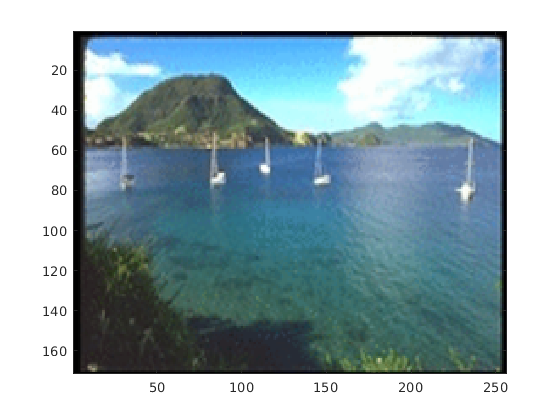
\includegraphics[width=0.8\textwidth]{images/Paysages67.png}
        \caption{\texttt{Paysages67.png}}
    \end{subfigure}
    \begin{subfigure}[c]{0.46\textwidth}
        \centering
        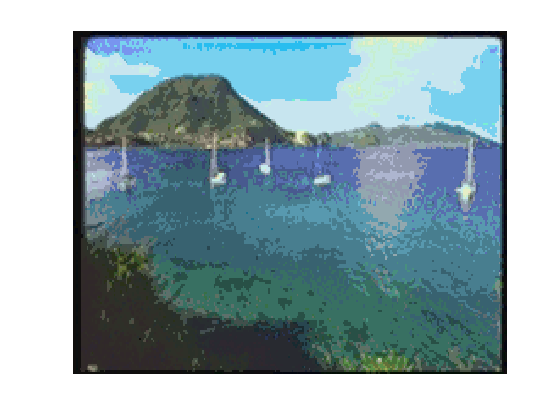
\includegraphics[width=0.8\textwidth]{images/Paysages67_quantifie.png}
        \caption{\texttt{Paysages67.png} quantifiée}
        \label{subfig:ex1_house}
    \end{subfigure}
    \begin{subfigure}[c]{0.46\textwidth}
        \centering
        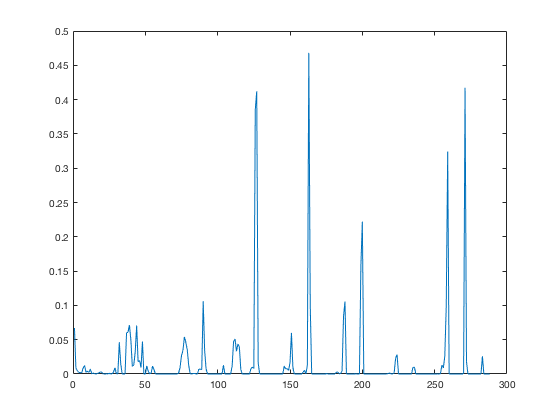
\includegraphics[width=0.8\textwidth]{images/Paysages67_histo.png}
        \caption{Histogramme de \texttt{Paysages67.png} quantifiée}
    \end{subfigure}
    \begin{subfigure}[c]{0.46\textwidth}
        \centering
        
\includegraphics[width=0.8\textwidth]{images/Paysages67_domi.png}
        \caption{Couleurs dominantes de \texttt{Paysages67.png}}
    \end{subfigure}

    \caption{Calcul d'histogrammes HSV sur \texttt{Paysages67.png} avec $nH=12$,
    $nS=3$, $nV=8$} 
    \label{fig:ex1_Paysages67}
\end{figure}

\begin{figure}[H]
    \centering
     
    \begin{subfigure}[c]{0.46\textwidth}
        \centering
        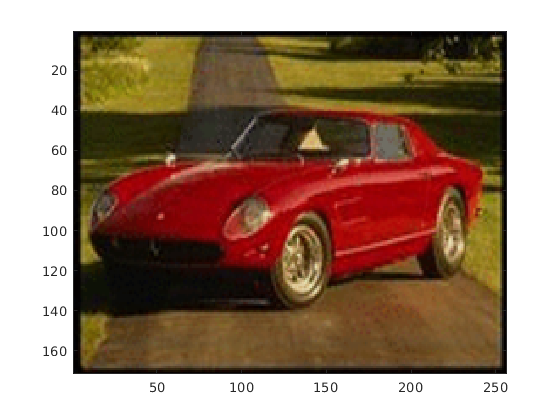
\includegraphics[width=0.8\textwidth]{images/Voitures76.png}
        \caption{\texttt{Voitures76.png}}
    \end{subfigure}
    \begin{subfigure}[c]{0.46\textwidth}
        \centering
        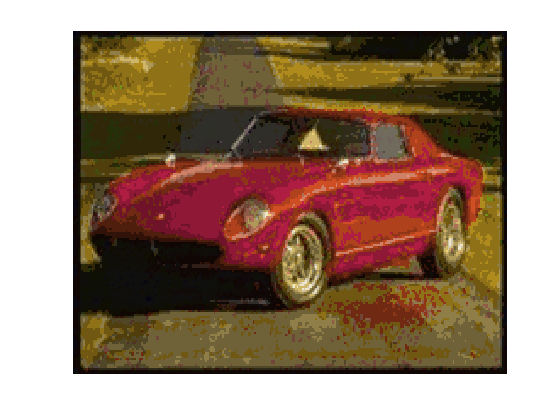
\includegraphics[width=0.8\textwidth]{images/Voitures76_quantifie.png}
        \caption{\texttt{Voitures76.png} quantifiée}
    \end{subfigure}
    \begin{subfigure}[c]{0.46\textwidth}
        \centering
        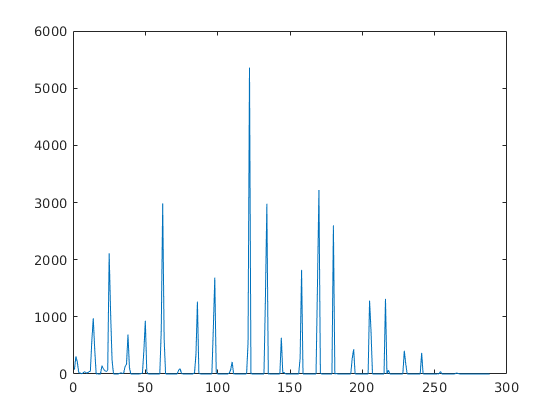
\includegraphics[width=0.8\textwidth]{images/Voitures76_histo.png}
        \caption{Histogramme de \texttt{Voitures76.png} quantifiée}
    \end{subfigure}
    \begin{subfigure}[c]{0.46\textwidth}
        \centering
        
\includegraphics[width=0.8\textwidth]{images/Voitures76_domi.png}
        \caption{Couleurs dominantes de \texttt{Voitures76.png}}
    \end{subfigure}

    \caption{Calcul d'histogrammes HSV sur \texttt{Voitures76.png}} 
    \label{fig:ex1_Voitures76}
\end{figure}

\begin{figure}[H]
    \centering
     
    \begin{subfigure}[c]{0.46\textwidth}
        \centering
        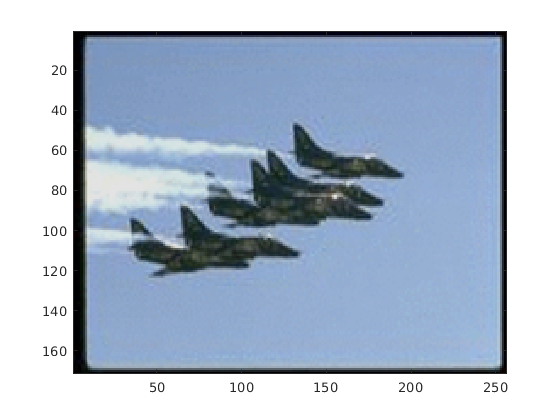
\includegraphics[width=0.8\textwidth]{images/Avions83.png}
        \caption{\texttt{Avions83.png}}
    \end{subfigure}
    \begin{subfigure}[c]{0.46\textwidth}
        \centering
        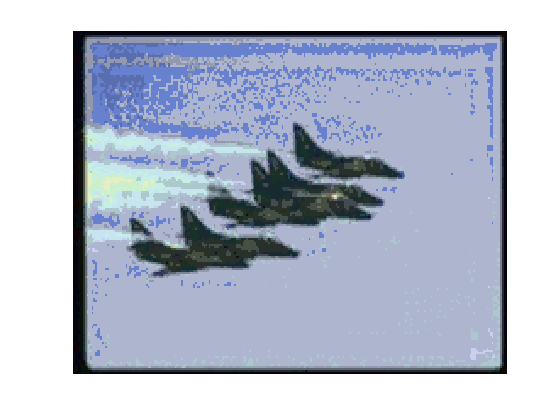
\includegraphics[width=0.8\textwidth]{images/Avions83_quantifie.png}
        \caption{\texttt{Avions83.png} quantifiée}
    \end{subfigure}
    \begin{subfigure}[c]{0.46\textwidth}
        \centering
        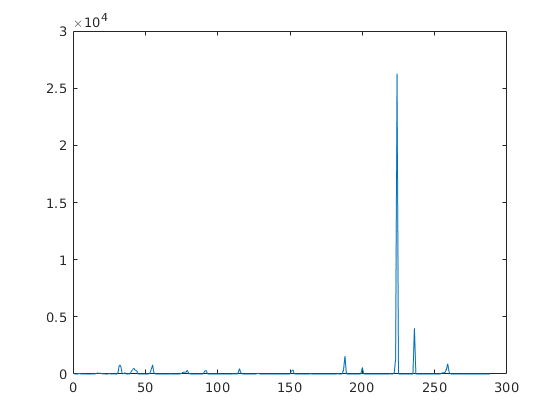
\includegraphics[width=0.8\textwidth]{images/Avions83_histo.png}
        \caption{Histogramme de \texttt{Avions83.png} quantifiée}
    \end{subfigure}
    \begin{subfigure}[c]{0.46\textwidth}
        \centering
        
\includegraphics[width=0.8\textwidth]{images/Avions83_domi.png}
        \caption{Couleurs dominantes de \texttt{Avions83.png}}
    \end{subfigure}

    \caption{Calcul d'histogrammes HSV sur \texttt{Avions83.png}} 
    \label{fig:ex1_Avions83}
\end{figure}

Nous faisons maintenant varier le nombre de bins de quantifications $nH$, $nS$
et $nV$ pour l'image \texttt{Paysages67.png}. Les résultats sont présentés dans la \figref{fig:ex1_var}.

\begin{figure}[H]
    \centering

    \begin{subfigure}[c]{0.8\textwidth}
        \centering
        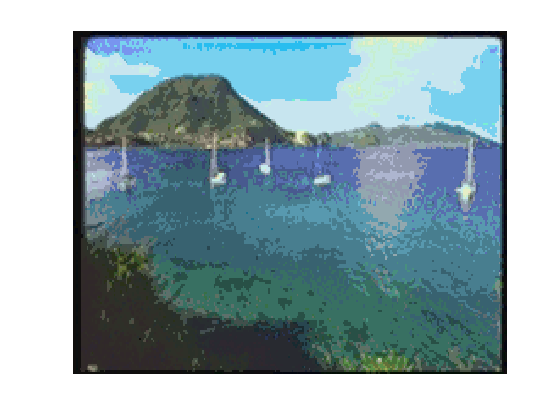
\includegraphics[width=0.46\textwidth]{images/Paysages67_quantifie.png}
        
\includegraphics[width=0.46\textwidth]{images/Paysages67_domi.png}
        \caption{$nH = 12$, $nS = 3$, $nV = 8$}
        \label{subfig:Paysages67_original}
    \end{subfigure}

    \begin{subfigure}[c]{0.8\textwidth}
        \centering
        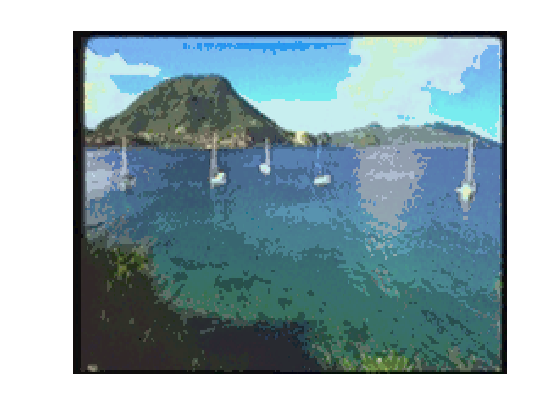
\includegraphics[width=0.46\textwidth]{images/Paysages67_quantifie_nHx10.png}
        
\includegraphics[width=0.46\textwidth]{images/Paysages67_domi_nHx10.png}
        \caption{$nH = 120$, $nS = 3$, $nV = 8$}
        \label{subfig:Paysages67_nHx10}
    \end{subfigure}

    \begin{subfigure}[c]{0.8\textwidth}
        \centering
        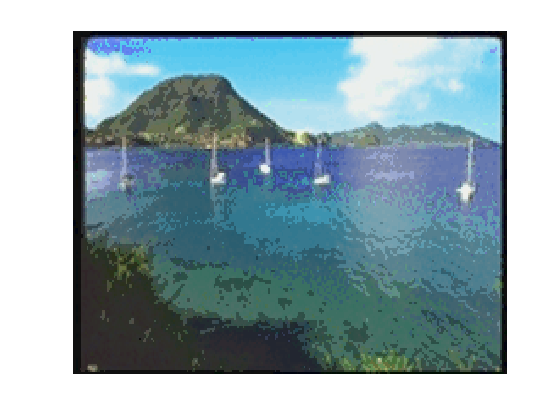
\includegraphics[width=0.46\textwidth]{images/Paysages67_quantifie_nSx10.png}
        
\includegraphics[width=0.46\textwidth]{images/Paysages67_domi_nSx10.png}
        \caption{$nH = 12$, $nS = 30$, $nV = 8$}
        \label{subfig:Paysages67_nSx10}
    \end{subfigure}

    \begin{subfigure}[c]{0.8\textwidth}
        \centering
        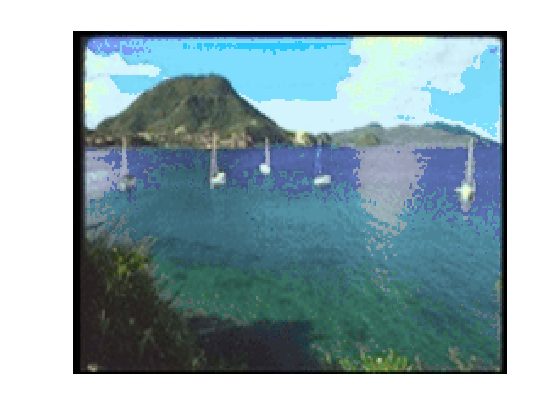
\includegraphics[width=0.46\textwidth]{images/Paysages67_quantifie_nVx10.png}
        
\includegraphics[width=0.46\textwidth]{images/Paysages67_domi_nVx10.png}
        \caption{$nH = 12$, $nS = 3$, $nV = 80$}
        \label{subfig:Paysages67_nVx10}
    \end{subfigure}

    \begin{subfigure}[c]{0.8\textwidth}
        \centering
        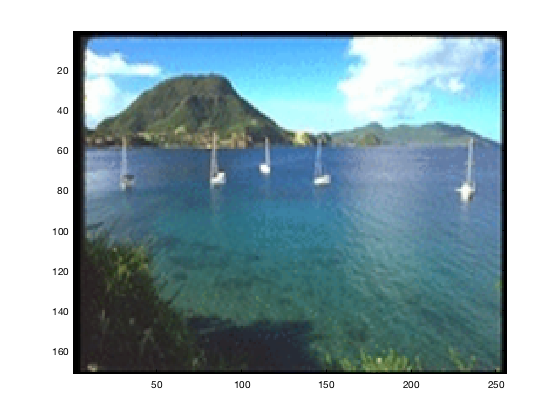
\includegraphics[width=0.46\textwidth]{images/Paysages67_quantifie_x10.png}
        
\includegraphics[width=0.46\textwidth]{images/Paysages67_domi_x10.png}
        \caption{$nH = 120$, $nS = 30$, $nV = 80$}
        \label{subfig:Paysages67_x10}
    \end{subfigure}

    \caption{Évolution de l'image \texttt{Paysages67.png} quantifiée en fonction
    des bins de quantification} 
    \label{fig:ex1_var}
\end{figure}

\newpage
\section*{Exercice 2 - Similarité entre images : recherche par le contenu}

Nous utilisons maintenant ce descripteur dans le cadre d'une application de
recherche par le contenu dans la base d'images fournie. \\

La similarité entre deux images est calculée par le produit scalaire entre leurs
histogrammes HSV normalisés. Nous calculons donc les histogrammes HSV pour
l'ensemble des images de la base, puis la matrice de similarité associée
(\figref{fig:ex2_matriceSim}).

\begin{figure}[H]
    \center
    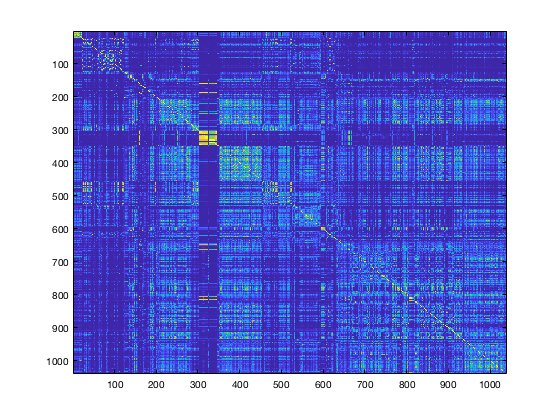
\includegraphics[width=0.6\textwidth]{images/matriceSim.png}
    \caption{Matrice de similarité pour l'ensemble de la base d'images}
    \label{fig:ex2_matriceSim}
\end{figure}

Nous effectuons désormais la recherche par similarité pour les images
\texttt{Liontigre1.png}, \texttt{Avions32.png}, \texttt{Paysages27.png}, et
\texttt{Voitures15.png}. Les résultats sont respectivement présentés dans les
figures \ref{fig:ex2_query350}, \ref{subfig:ex2_query50},
\ref{subfig:ex2_query550}, et \ref{subfig:ex2_query950}.

\begin{figure}[H]
    \center
    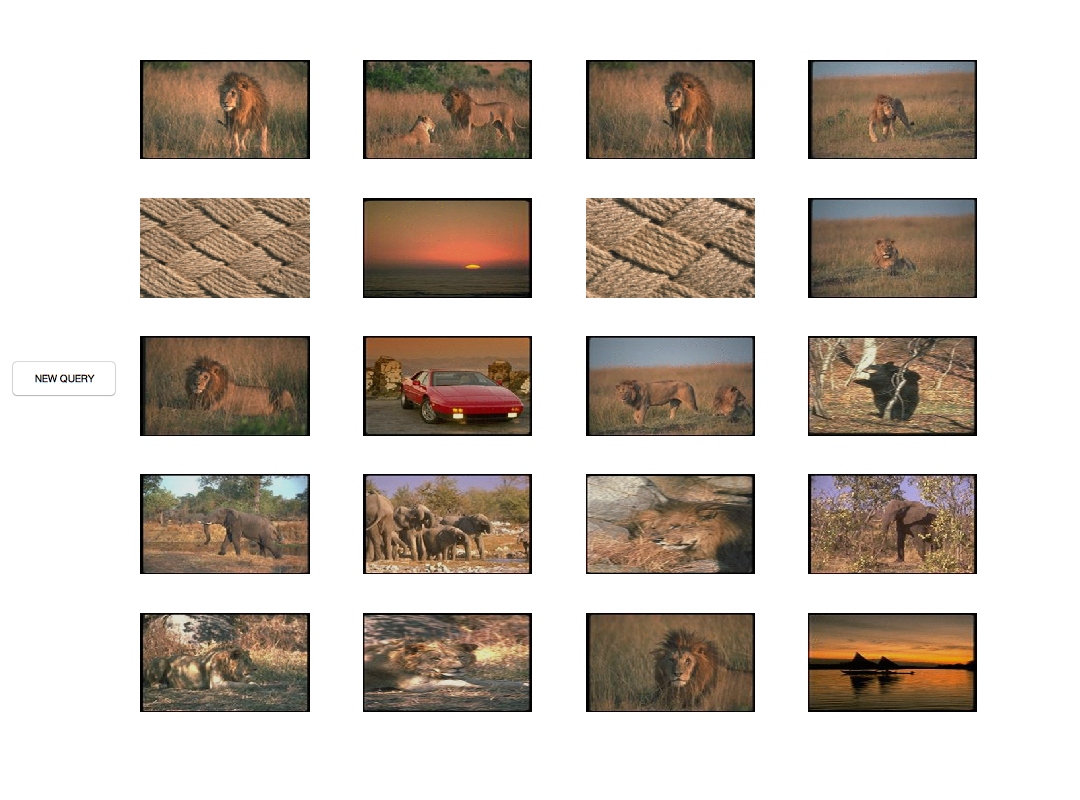
\includegraphics[width=0.8\textwidth]{images/query350.png}
    \caption{Résultat de la recherche par similarité pour l'image
    \texttt{Liontigre1.png}}
    \label{fig:ex2_query350}
\end{figure}

\begin{figure}[H]
    \centering
     
    \begin{subfigure}[c]{0.6\textwidth}
        \centering
        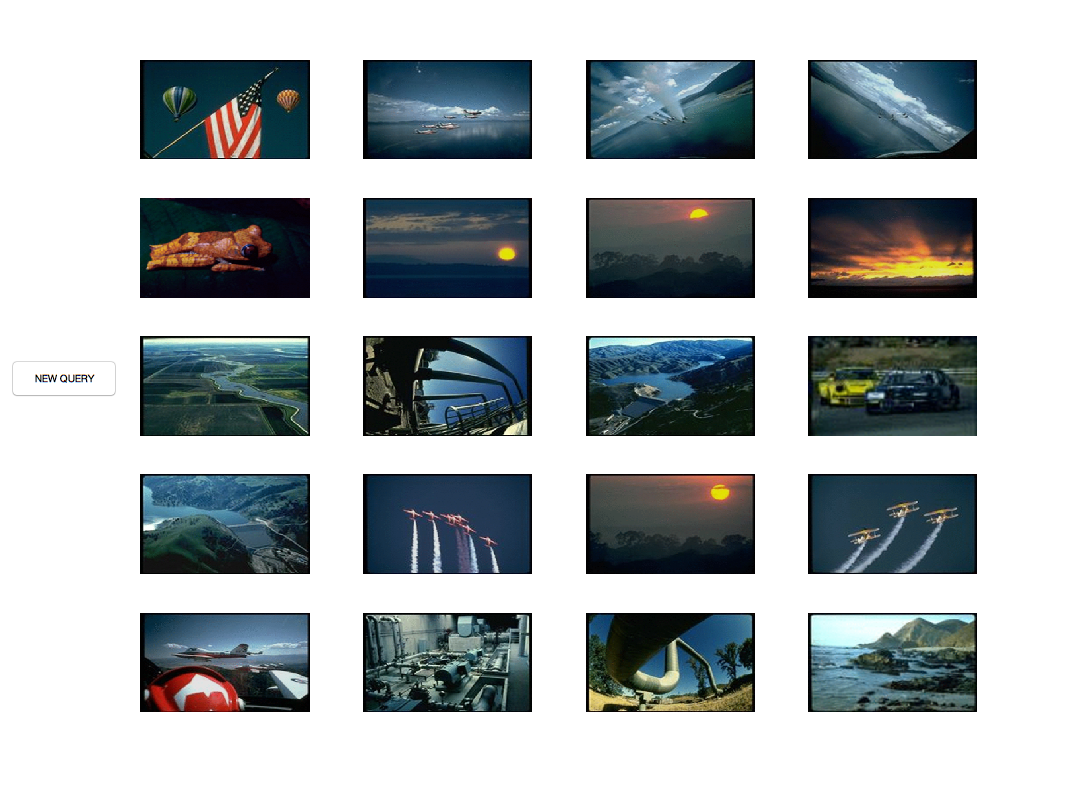
\includegraphics[width=\textwidth]{images/query50.png}
        \caption{Résultat de la recherche par similarité pour l'image
        \texttt{Avions32.png}}
        \label{subfig:ex2_query50}
    \end{subfigure}
    \begin{subfigure}[c]{0.6\textwidth}
        \centering
        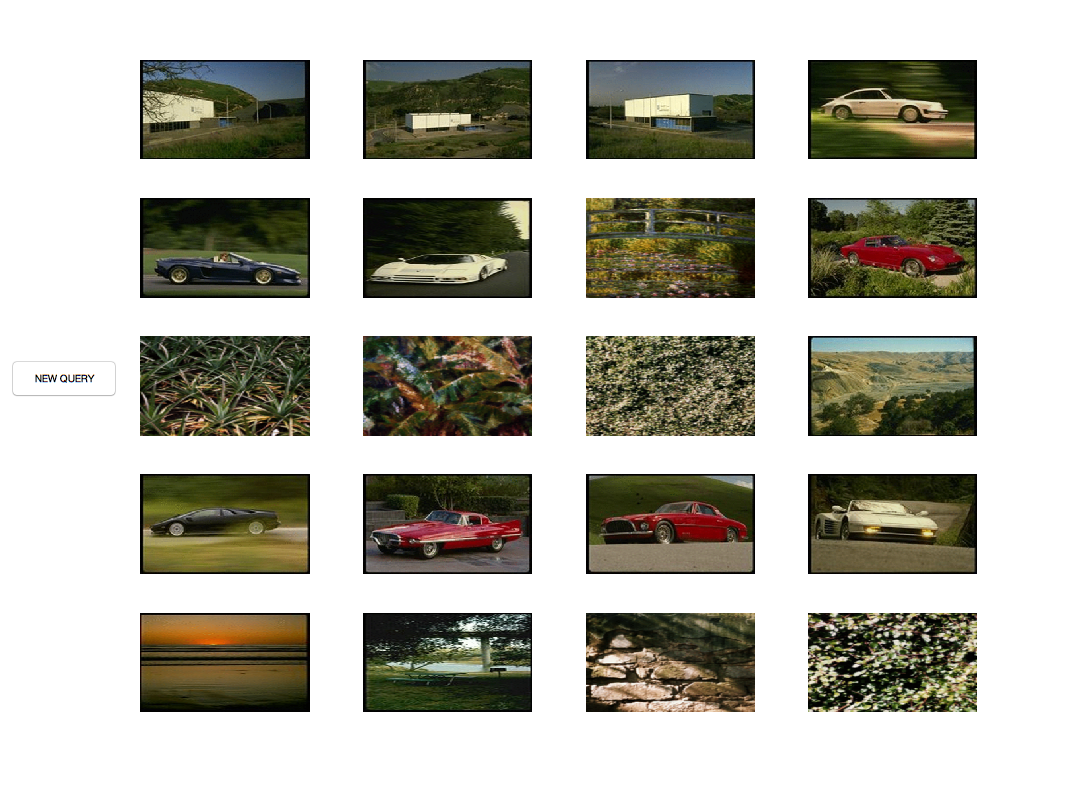
\includegraphics[width=\textwidth]{images/query550.png}
        \caption{Résultat de la recherche par similarité pour l'image
    \texttt{Paysages27.png}}
        \label{subfig:ex2_query550}
    \end{subfigure}
    \begin{subfigure}[c]{0.6\textwidth}
        \centering
        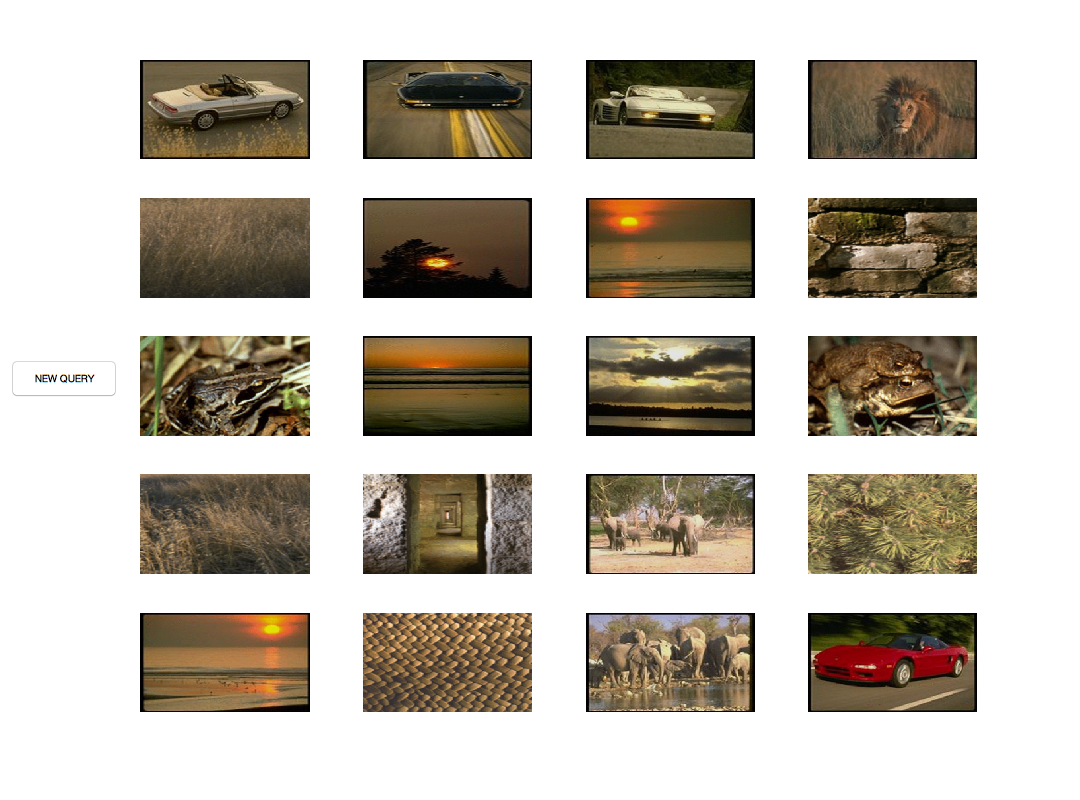
\includegraphics[width=\textwidth]{images/query950.png}
        \caption{Résultat de la recherche par similarité pour l'image
    \texttt{Voitures15.png}}
        \label{subfig:ex2_query950}
    \end{subfigure}

    \caption{Résultat de recherches par similarité pour quelques images de la
    base}
    \label{fig:ex2_queries}

\end{figure}

Nous observons sur la \figref{fig:ex2_queries} que la recherche par contenu
basée sur le descripteur couleur renvoie des images dont la signature
colorimétrique est similaire à celle de l'image passée en entrée. Cependant, le
contenu sémantique n'est pas forcément le même. Par exemple, la montgolfière de
la \figref{subfig:ex2_query50} (en haut à gauche) est assimilée, entre autres,
à des couchers de soleil, des rivières, et à des tuyaux.

Ce dernier fait met en évidence les limitations de cette approche brute basée
sur la similarité colorimétrique. En effet, le descripteur utilisé considère
seulement la signature globale (l'histogramme couleur) de l'image mais ne tient
pas compte de la notion de spatialité. Il est donc impossible d'effectuer une
recherche par catégories sémantiques (par exemple retrouver les images contenant
des lions ou des tigres dans la base).

\end{document}
